\documentclass[twocolumn, 10pt]{article} % 全局字体大小设为12pt

% 导入 ctex 包以支持中文
\usepackage[UTF8]{ctex}
\usepackage{courier} % 用于设置代码字体

% 设置页面边距
\usepackage{geometry}
\geometry{left=2cm,right=2cm,top=2.5cm,bottom=2.5cm}
\usepackage{amsthm}

\usepackage{listings} % 用于显示代码
\usepackage{color}

% 自定义带编号且斜体内容的 remark 环境
\theoremstyle{remark}
\newtheorem{remark}{Remark}

% 通过\textit命令让内容显示为斜体
\newenvironment{myremark}
  {\begin{remark}\itshape}
  {\end{remark}}


% 其他常用包
\usepackage{graphicx}   % 插入图片
\usepackage{amsmath}    % 数学公式
\usepackage{amssymb}    % 数学符号
\usepackage{hyperref}   % 超链接
\usepackage{enumitem}   % 引入 enumitem 包用于自定义列表
\usepackage{array} % 提供表格增强功能
\usepackage{stfloats} % 支持双栏排版中的浮动对象


\usepackage{xcolor} % 用于设置文本和背景颜色
\usepackage{times} % 设置全局字体为 Times New Roman,或者根据需求选择其他字体
% 表格字体设置
\usepackage{etoolbox}

% 导入titlecaps宏包
\usepackage{titlecaps}

\definecolor{codegray}{rgb}{0.5,0.5,0.5}
\definecolor{codeblue}{rgb}{0.25,0.5,0.75}
\definecolor{codepurple}{rgb}{0.58,0,0.82}

\lstdefinestyle{mystyle}{
    backgroundcolor=\color{white},   
    commentstyle=\color{codegray},
    keywordstyle=\color{codeblue},
    numberstyle=\tiny\color{codegray},
    stringstyle=\color{codepurple},
    basicstyle=\ttfamily\scriptsize, % 调整代码字体大小为 \scriptsize
    breakatwhitespace=false,         
    breaklines=true,                 
    captionpos=b,                    
    keepspaces=true,                 
    numbers=left,                    
    numbersep=5pt,                  
    showspaces=false,                
    showstringspaces=false,
    showtabs=false,                  
    tabsize=2
}

\lstset{style=mystyle}


% 自定义命令将标题首字母大写,其他单词小写
\Addlcwords{a an the of and in on at to with by for from}
\newcommand{\capitalizeTitle}[1]{\titlecap{#1}}

% 设置标题格式
\usepackage{titlesec}
\titleformat{\section}
  {\normalfont\Large\bfseries}
  {\thesection}{1em}{\capitalizeTitle}

\titleformat{\subsection}
  {\normalfont\large\bfseries}
  {\thesubsection}{1em}{\capitalizeTitle}

\titleformat{\subsubsection}
  {\normalfont\normalsize\bfseries}
  {\thesubsubsection}{1em}{\capitalizeTitle}









\AtBeginEnvironment{tabular}{\small} % 将表格内字体设为比正文小1号


% 定义浅黄色
\definecolor{lightyellow}{rgb}{1.0, 1.0, 0.88}

\begin{document}

% 标题
\title{Asynchronous Methods for Deep Reinforcement Learning}
\author{作者姓名}
\date{\today}
\maketitle
% 摘要

\section{论文的创新点与效果}

\subsection{创新点}

论文《Asynchronous Methods for Deep Reinforcement Learning》的主要创新点包括:

\begin{enumerate}
    \item \textbf{异步并行执行}:
    \begin{itemize}
        \item 论文提出了一种异步并行执行的框架,在此框架下,多个智能体在多个环境实例上并行执行。与传统的经验回放(experience replay)不同,这种方法能够使得数据的去相关性更强,并且能够在没有经验回放的情况下实现稳定的深度强化学习。
        \item 这种异步并行方法显著减少了对硬件的要求,实现了在普通多核CPU上训练深度强化学习模型,而无需依赖于GPU或大规模分布式计算架构。
    \end{itemize}
    
    \item \textbf{适用于多种强化学习算法}:
    \begin{itemize}
        \item 该方法不仅适用于基于值的方法(如Q-learning),还可以应用于策略梯度方法(如Actor-Critic)。这使得该方法在不同类型的任务中表现出很高的通用性,既可以用于离策略学习,也可以用于在策略学习。
        \item 通过引入异步优势Actor-Critic (A3C) 方法,该框架进一步提高了在复杂任务(如2D和3D游戏)的表现,尤其是在具有连续动作空间和视觉输入的任务中表现尤为突出。
    \end{itemize}
    
    \item \textbf{训练速度和资源利用效率}:
    \begin{itemize}
        \item 实验结果显示,异步方法在多个Atari 2600游戏上,使用16个CPU核心训练的速度比基于GPU的DQN方法更快,并且达到了相同甚至更好的性能。
        \item 异步优势Actor-Critic (A3C) 方法在训练时间上具有显著优势,能够在较短的时间内达到甚至超越当前最先进的强化学习算法的表现,尤其是在没有GPU支持的情况下。
    \end{itemize}
\end{enumerate}

\subsection{采用本论文提出的方法后的效果}

\begin{enumerate}
    \item \textbf{稳定性和训练速度的提升}:
    \begin{itemize}
        \item 异步并行执行的设计能够显著提高强化学习的稳定性,减少了传统在线强化学习中的不稳定性问题,尤其是与深度神经网络结合时。
        \item 异步方法使得多个智能体可以同时探索不同的状态空间,从而加快了训练过程,并且能够更快地收敛到较优策略。
    \end{itemize}
    
    \item \textbf{硬件资源需求的降低}:
    \begin{itemize}
        \item 由于不依赖于GPU或大规模的分布式架构,该方法可以在普通的多核CPU上实现高效的训练,这使得深度强化学习的应用更加普及和易于实施。
    \end{itemize}
    
    \item \textbf{更广泛的应用领域}:
    \begin{itemize}
        \item 该方法不仅在Atari游戏中表现出色,还成功应用于更为复杂的任务,如3D迷宫导航和连续动作控制任务。这证明了该方法在不同类型任务和不同输入空间下的广泛适用性。
    \end{itemize}
    
    \item \textbf{较高的数据效率和探索效率}:
    \begin{itemize}
        \item 异步方法通过多智能体并行探索大大提高了数据利用效率,并且在不使用经验回放的情况下,也能稳定高效地学习,适应性更强。
    \end{itemize}
\end{enumerate}

这些创新点和效果使得该方法成为深度强化学习领域的重要突破,特别是在资源受限的环境中,提供了一种高效、稳定的解决方案。


\section{A2C Algorithm 解读}
\begin{figure}[h!]
    \centering
    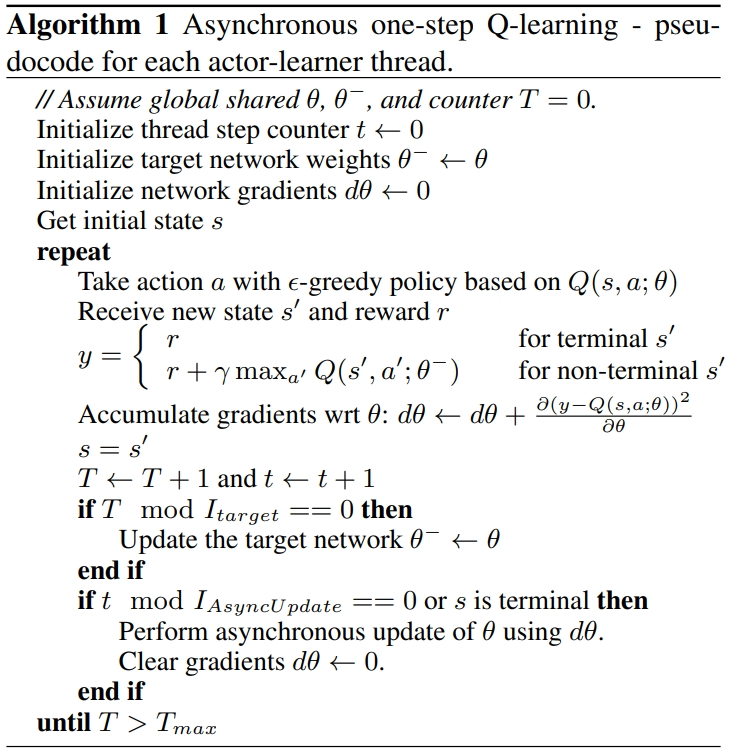
\includegraphics[width=\columnwidth]{a2c_alg.png} % 使用单栏宽度的图片
    \caption{A2C算法示意图}
    \label{fig:a2c}
\end{figure}
该算法图\ref{fig:a2c}展示了\textbf{异步一步Q-learning(Asynchronous One-Step Q-learning)}的伪代码,用于每个 actor-learner 线程。以下是对这个算法的详细解读:

\subsection{全局参数的假设}
\begin{itemize}
    \item \textbf{全局共享参数}:
    \begin{itemize}
        \item \( \theta \):表示当前的全局神经网络权重,它们在多个线程间共享。
        \item \( \theta^- \):表示目标网络(target network)的权重。目标网络的权重 \( \theta^- \) 是 \(\theta\) 的一个延迟副本,用于稳定Q值的更新。
        \item \( T \):一个全局计数器,用来跟踪所有线程执行的总步数。
    \end{itemize}
\end{itemize}

\subsection{线程初始化}
\begin{itemize}
    \item 初始化线程步骤计数器 \( t \leftarrow 0 \)。
    \item 将目标网络的权重初始化为当前的网络权重,即 \( \theta^- \leftarrow \theta \)。
    \item 初始化网络梯度 \( d\theta \leftarrow 0 \)。这个变量用于累积在每个时间步上的梯度。
    \item 获取初始状态 \( s \)。
\end{itemize}

\subsection{主循环 (repeat)}
主循环中的每个线程执行以下步骤,直到全局计数器 \( T \) 超过 \( T_{max} \):

\begin{itemize}
    \item \textbf{选择动作 \( a \)}:
    \begin{itemize}
        \item 通过 \(\epsilon\)-贪心策略(\(\epsilon\)-greedy policy)基于 \( Q(s, a; \theta) \) 选择动作。这个策略通过一定概率选择随机动作(探索),或者选择当前估计最优的动作(利用)。
    \end{itemize}
    
    \item \textbf{执行动作并接收新状态 \( s' \) 和奖励 \( r \)}:
    \begin{itemize}
        \item 执行动作 \( a \),接收环境返回的下一状态 \( s' \) 和即时奖励 \( r \)。
    \end{itemize}
    
    \item \textbf{计算目标值 \( y \)}:
    \begin{itemize}
        \item 如果 \( s' \) 是终止状态(terminal state),目标值 \( y = r \)。
        \item 如果 \( s' \) 不是终止状态,目标值 \( y = r + \gamma \max_{a'} Q(s', a'; \theta^-) \),其中 \( \gamma \) 是折扣因子。
    \end{itemize}
    
    \item \textbf{累积梯度 \( d\theta \)}:
    \begin{itemize}
        \item 计算相对于 \( \theta \) 的梯度,并累积到 \( d\theta \) 中:
        \[
        d\theta \leftarrow d\theta + \frac{\partial (y - Q(s, a; \theta))^2}{\partial \theta}
        \]
        这个累积过程允许在多个时间步上聚合梯度,从而实现更有效的更新。
    \end{itemize}
    
    \item \textbf{更新状态和计数器}:
    \begin{itemize}
        \item 将当前状态更新为下一状态 \( s \leftarrow s' \)。
        \item 更新全局步数计数器 \( T \leftarrow T + 1 \) 以及线程局部的步骤计数器 \( t \leftarrow t + 1 \)。
    \end{itemize}
    
    \item \textbf{目标网络的更新}:
    \begin{itemize}
        \item 每当 \( T \mod I_{target} == 0 \) 时,更新目标网络的权重 \( \theta^- \leftarrow \theta \),其中 \( I_{target} \) 是更新目标网络的间隔。
    \end{itemize}
    
    \item \textbf{异步更新 \( \theta \)}:
    \begin{itemize}
        \item 如果 \( t \mod I_{AsyncUpdate} == 0 \) 或 \( s \) 是终止状态,则执行异步更新:
        \begin{itemize}
            \item 使用累积的梯度 \( d\theta \) 来更新全局网络的权重 \( \theta \)。
            \item 清空累积的梯度 \( d\theta \leftarrow 0 \)。
        \end{itemize}
    \end{itemize}
\end{itemize}

\subsection{终止条件}
主循环继续,直到全局计数器 \( T \) 超过最大步数 \( T_{max} \)。

\subsection{主要特点与优势}
\begin{itemize}
    \item \textbf{异步更新}:通过异步更新,多个线程可以并行工作而不需要等待其他线程完成,使得训练更加高效。
    \item \textbf{目标网络的使用}:目标网络 \( \theta^- \) 的使用有助于稳定训练,减少了在Q值更新中的高方差问题。
    \item \textbf{\(\epsilon\)-贪心策略}:在动作选择中采用\(\epsilon\)-贪心策略,平衡了探索和利用的关系,确保了智能体可以探索新的动作策略,同时也利用当前最优的策略。
\end{itemize}

\subsection{整体流程的总结}
该算法是通过多个线程并行运行,使用共享的全局网络权重进行异步更新。这种异步方式使得算法在多核处理器上可以更加高效地运行,同时通过目标网络和梯度累积等技术来确保训练的稳定性和高效性。这种方法广泛应用于大型的深度强化学习任务中,如游戏AI的训练。


\appendix
\section{Python代码解读:A2C算法实现}

a2c.py实现了 A2C(Asynchronous Advantage Actor-Critic)算法的核心部分。以下是对这段代码的详细解读,以及它与 A2C 算法伪代码之间的对应关系。

\subsection{Model 类的定义}
\texttt{Model} 类用于管理模型的创建、训练、保存和加载。它包括初始化函数 \texttt{\_\_init\_\_}、训练函数 \texttt{train()}、以及保存和加载模型的函数。

\subsubsection{\_\_init\_\_ 函数}
\begin{itemize}
    \item \textbf{policy}: 初始化 \texttt{step\_model} 和 \texttt{train\_model} 两个模型。 \texttt{step\_model} 用于采样动作,\texttt{train\_model} 用于训练网络。两个模型共用相同的网络结构,但是 \texttt{train\_model} 是基于批次(batch)处理的。
    \item \textbf{占位符(Placeholders)}: 定义了三个主要的占位符,用于存储动作(\texttt{A})、优势函数(\texttt{ADV})、回报(\texttt{R})以及学习率(\texttt{LR})。
    \item \textbf{损失函数(Loss)}: 计算总损失,包括策略损失(Policy Gradient Loss)、熵损失(Entropy Loss,用于增强探索)和价值损失(Value Function Loss)。总损失计算如下:
    \[
    \text{loss} = \text{pg\_loss} - \text{entropy} \times \text{ent\_coef} + \text{vf\_loss} \times \text{vf\_coef}
    \]
    \item \textbf{梯度计算和参数更新}:
    \begin{itemize}
        \item 使用 \texttt{tf.gradients} 计算损失函数关于模型参数的梯度。
        \item 如果设置了 \texttt{max\_grad\_norm},则对梯度进行裁剪(gradient clipping)以避免梯度爆炸。
        \item 使用 \texttt{RMSPropOptimizer} 优化器更新参数。
    \end{itemize}
\end{itemize}

\subsubsection{train 函数}
\begin{itemize}
    \item \textbf{计算优势函数(Advantage Calculation)}: \texttt{adv = R + $\gamma$ V(s') - V(s)},在实际计算中,\texttt{adv} 被简化为 \texttt{rewards - values}。
    \item \textbf{训练步骤}:
    \begin{itemize}
        \item 将观察(\texttt{obs})、动作(\texttt{actions})、优势(\texttt{ADV})、回报(\texttt{R})和学习率(\texttt{LR})等数据映射到 \texttt{train\_model} 中。
        \item 执行 TensorFlow 会话以更新策略和价值函数,并返回损失值(\texttt{policy\_loss}、\texttt{value\_loss} 和 \texttt{policy\_entropy})。
    \end{itemize}
\end{itemize}

\subsection{learn 函数}
\texttt{learn} 函数是 A2C 算法的主入口,负责训练模型。
\begin{itemize}
    \item \textbf{模型实例化}: 创建 \texttt{Model} 类的实例,其中包含了策略网络 \texttt{policy} 和环境 \texttt{env}。
    \item \textbf{经验收集}:
    \begin{itemize}
        \item 使用 \texttt{Runner} 类来管理与环境的交互,收集多个时间步的观察、状态、奖励、掩码、动作和价值。
    \end{itemize}
    \item \textbf{训练过程}:
    \begin{itemize}
        \item 在每次更新中,通过 \texttt{runner.run()} 收集一批次的经验数据,然后使用 \texttt{model.train()} 函数进行训练。
    \end{itemize}
    \item \textbf{记录与日志}:
    \begin{itemize}
        \item 每隔一段时间,计算并记录关键指标,例如策略熵、价值损失、解释方差(explained variance)等。
    \end{itemize}
\end{itemize}

\subsection{与A2C伪代码的对应关系}
\begin{itemize}
    \item \textbf{初始化}:
    \begin{itemize}
        \item 在伪代码中,初始化全局模型参数、目标网络权重和计数器。代码中,\texttt{\_\_init\_\_} 函数负责初始化模型参数,创建 \texttt{step\_model} 和 \texttt{train\_model}。
    \end{itemize}
    \item \textbf{执行与更新}:
    \begin{itemize}
        \item 伪代码的主循环中执行动作、计算损失、更新模型参数。在代码中,\texttt{train} 函数执行这些任务,而 \texttt{learn} 函数则负责管理整个训练过程,包括调用 \texttt{train} 函数进行参数更新。
    \end{itemize}
    \item \textbf{梯度计算和裁剪}:
    \begin{itemize}
        \item 伪代码中提到梯度计算和裁剪(clipping),在代码中由 \texttt{tf.gradients} 和 \texttt{tf.clip\_by\_global\_norm} 实现。
    \end{itemize}
    \item \textbf{记录与日志}:
    \begin{itemize}
        \item 在伪代码中,通常通过 \texttt{if} 条件控制记录和日志打印。代码中使用 \texttt{logger} 模块记录模型训练过程中的各种信息。
    \end{itemize}
\end{itemize}


\section{policy}
\begin{itemize}
    \item \textbf{policy}:policy(策略) 是一个核心概念,它指的是智能体(agent)在给定状态(state)下采取动作(action)的规则或方法。策略的目标是最大化长期回报(通常称为累积奖励或回报),这意味着智能体通过学习或优化其策略,以在未来的时间内获得尽可能高的奖励。
\begin{itemize}
    \item \textbf{	确定性策略(Deterministic Policy)}:在确定性策略下,策略函数  $\pi \left( s \right)$ 直接输出一个具体的动作  即在给定状态  $s$ 时,智能体总是选择同一个动作。\textbf{数学表示}:  $\pi \left(s\right) = a$
\end{itemize}
\begin{itemize}
    \item \textbf{	随机性策略(Stochastic Policy)}:在随机性策略下,策略函数  $\pi \left( a|s \right)$   输出的是在给定状态  $s$ 时采取某个动作 $a$ 的概率分布。智能体根据这个分布随机选择动作。\textbf{数学表示}:  $\pi\left(a|s\right)=P\left(a|s\right)$
\end{itemize}
\end{itemize}

\section{动作价值函数与状态价值函数的区别}

动作价值函数(Action Value Function)和状态价值函数(State Value Function)是强化学习中的两个重要概念,它们在评估不同策略时提供了不同的信息。以下是它们的区别和联系:

\subsection{定义}

\begin{itemize}
    \item \textbf{动作价值函数 $Q(s, a)$}: \\
    动作价值函数 \(Q(s, a)\) 表示在给定状态 \(s\) 下,采取某个特定动作 \(a\) 后,未来所能获得的累积回报的期望值。它既考虑了当前的即时奖励 \(r_t\),也考虑了未来各个时刻的回报,并假设之后将按照策略 \(\pi\) 继续行动。

    数学上定义为:
    $$
    Q^\pi(s, a) = \mathbb{E} \left[ R_t \mid s_t = s, a_t = a \right]
    $$
    其中,$ R_t = r_t + \gamma r_{t+1} + \gamma^2 r_{t+2} + \dots = \sum_{k=0}^{\infty} \gamma^k r_{t+k} $,表示从当前时刻 \(t\) 开始的累积回报。

    \item \textbf{状态价值函数 \(V(s)\)}: \\
    状态价值函数 \(V(s)\) 表示在给定状态 \(s\) 下,按照某个策略 \(\pi\) 继续行动时,未来所能获得的累积回报的期望值。与动作价值函数不同,状态价值函数只考虑当前状态,不考虑特定的动作。

    数学上定义为:
    $$
    V^\pi(s) = \mathbb{E}_\pi \left[ R_t \mid s_t = s \right]
    $$
\end{itemize}

\subsection{公式关系}
 动作价值函数和状态价值函数之间存在以下关系:
$$
Q^\pi(s, a) = \mathbb{E} \left[ r_t + \gamma V^\pi(s_{t+1}) \mid s_t = s, a_t = a \right]
$$


这意味着 \(Q(s, a)\) 可以分解为当前时刻的即时奖励 \(r_t\) 和下一个状态的状态价值函数 \(V(s_{t+1})\) 的加权和。

\subsection{应用场景}

\begin{itemize}
    \item \textbf{动作价值函数 \(Q(s, a)\)}: 动作价值函数通常用于策略改进,例如在 Q-learning 中,智能体通过选择使 \(Q(s, a)\) 最大化的动作 \(a\) 来确定最优策略。因此,动作价值函数在决定每个状态下的具体动作时尤为重要。

    \item \textbf{状态价值函数 \(V(s)\)}: 状态价值函数通常用于策略评估,它提供了策略在不同状态下整体表现的衡量。状态价值函数可以用于评估某个策略的优劣,而不必涉及具体的动作选择。
\end{itemize}

\subsection{直观理解}

\textbf{状态价值函数关注的是“在这个状态下总体上有多好”,不关心具体采取哪个动作。动作价值函数关注的是“在这个状态下采取这个动作有多好”},需要结合特定的动作来评估回报。

\subsection{例子}

假设一个棋盘游戏中,某个位置 \(s\) 是一个状态,可能的动作包括“向左移动”或“向右移动”:
\begin{itemize}
    \item \textbf{状态价值函数 \(V(s)\)}: 可能表示在位置 \(s\) 上,继续游戏并最终获胜的期望概率。
    \item \textbf{动作价值函数 \(Q(s, \text{左移})\)}: 可能表示从位置 \(s\) 向左移动后,继续游戏并最终获胜的期望概率。
\end{itemize}

\subsection{总结}

\textbf{状态价值函数衡量状态的好坏,动作价值函数衡量在某个状态下采取某个具体动作的好坏}。两者在强化学习中密切相关,但在不同的算法和应用场景中扮演不同的角色。


\section{Value-based和Policy-based强化学习}

在强化学习(Reinforcement Learning, RL)中,\textbf{Value-based} 和 \textbf{Policy-based} 是两种主要的方法,用于解决不同类型的决策问题。它们在学习策略(policy)和评估策略的方式上有着本质的区别。

\subsection{Value-based 强化学习}

\textbf{Value-based方法}的核心是估计某种形式的“价值函数”,并通过最大化这个价值函数来导出最优策略。常见的价值函数有两种:

\begin{itemize}
    \item \textbf{状态价值函数 \( V(s) \)}:表示在状态 \( s \) 下执行策略 \( \pi \) 所能获得的期望累积回报。
    \item \textbf{状态-动作价值函数 \( Q(s, a) \)}:表示在状态 \( s \) 下采取动作 \( a \) 并随后遵循策略 \( \pi \) 所能获得的期望累积回报。
\end{itemize}

\textbf{典型算法}:

\begin{itemize}
    \item \textbf{Q-learning}:Q-learning 是一种无模型的强化学习算法,通过迭代更新Q值来学习最优策略。Q-learning 直接更新 Q 值并根据最大化 Q 值来选择动作,即学习的是最优的 Q 函数。
  
    \item \textbf{DQN(Deep Q-Network)}:DQN 是一种结合深度学习的 Q-learning 方法,用神经网络来逼近 Q 值函数,适用于高维状态空间。
\end{itemize}

\textbf{优缺点}:
\begin{itemize}
    \item \textbf{优点}:适用于离散的动作空间,计算简单,易于实现。
    \item \textbf{缺点}:在高维连续动作空间中效果不佳,策略导出的动作选择往往基于最大化Q值,容易导致“贪心”策略。
\end{itemize}

\subsection{Policy-based 强化学习}

\textbf{Policy-based方法}直接学习一个策略(policy),即动作选择的概率分布。策略可以是确定性的,也可以是随机性的。这里不涉及显式的价值函数估计。

\begin{itemize}
    \item \textbf{策略函数 \( \pi(a|s) \)}:表示在状态 \( s \) 下选择动作 \( a \) 的概率。
\end{itemize}

\textbf{典型算法}:

\begin{itemize}
    \item \textbf{REINFORCE}:一种基于梯度的策略优化算法,通过采样策略梯度来更新策略的参数。每个回合后,根据累积的回报来调整策略。

    \item \textbf{Actor-Critic}:结合了价值函数和策略的方法,Actor 负责选择动作(即策略),Critic 评估动作的好坏(即价值函数)。通过Critic提供的反馈来更新Actor的策略。

    \item \textbf{PPO(Proximal Policy Optimization)}:PPO 是一种较新的策略优化算法,通过限制更新幅度来保持策略更新的稳定性,广泛应用于复杂强化学习任务。
\end{itemize}

\textbf{优缺点}:
\begin{itemize}
    \item \textbf{优点}:适用于连续动作空间,策略直接输出动作的概率,能处理更复杂的策略表达。
    \item \textbf{缺点}:训练不稳定,需要更高的计算资源,容易陷入局部最优。
\end{itemize}

\subsection{总结}

\begin{itemize}
    \item \textbf{Value-based方法}侧重于学习价值函数,然后基于价值函数导出最优策略。典型代表是Q-learning和DQN。
    \item \textbf{Policy-based方法}直接学习策略,通过优化策略的期望回报来获得最优策略。典型代表是REINFORCE、Actor-Critic和PPO。
\end{itemize}

在实际应用中,很多强化学习算法会结合这两种方法的优点,形成混合的方法,如Actor-Critic 就是将价值函数和策略结合起来的方法。

\section{动作价值函数的Q-learning更新机制}

在强化学习(Reinforcement Learning)中,动作价值函数(Action Value Function) \( Q(s, a) \) 是评估在状态 \( s \) 下采取动作 \( a \) 后,智能体未来预期能够获得的累积回报的一个重要函数。为了计算和优化 \( Q(s, a) \),通常使用基于值的无模型方法(model-free methods),其中最典型的是 Q-learning 算法。

在 Q-learning 中,动作价值函数 \( Q(s, a; \theta) \) 通常由一个参数化的函数近似器(例如神经网络)来表示,参数为 \( \theta \)。为了使这个近似的动作价值函数逐步逼近最优动作价值函数 \( Q^*(s, a) \),我们通过反复更新参数 \( \theta \) 来改进 \( Q(s, a; \theta) \) 的估计。

Q-learning 的核心在于通过最小化一系列损失函数来更新参数 \( \theta \)。具体而言,第 \( i \) 次更新时使用的损失函数 \( L_i(\theta_i) \) 定义为:
$$
L_i(\theta_i) = \mathbb{E} \left( r + \gamma \max_{a'} Q(s', a'; \theta_{i-1}) - Q(s, a; \theta_i) \right)^2
$$

在这个公式中:
\begin{itemize}
    \item \( s' \) 是在状态 \( s \) 下采取动作 \( a \) 后到达的下一个状态。
    \item \( r \) 是即时奖励。
    \item \( \gamma \) 是折扣因子,用于平衡即时奖励和未来奖励的相对重要性。
    \item \( \max_{a'} Q(s', a'; \theta_{i-1}) \) 表示在下一个状态 \( s' \) 下,根据前一次迭代的参数 \( \theta_{i-1} \) 选择最优动作 \( a' \) 后的预期回报。
\end{itemize}

通过最小化损失函数 \( L_i(\theta_i) \),Q-learning 逐步调整参数 \( \theta \),使得 \( Q(s, a; \theta_i) \) 更加精确地逼近目标值 \( r + \gamma \max_{a'} Q(s', a'; \theta_{i-1}) \),从而优化动作选择策略。这个过程通过多次迭代实现,最终使智能体能够在每个状态下选择最优动作,以最大化未来的累积回报。


\begin{myremark}
在“基于值的无模型方法”中,“无模型”指的是这些方法不依赖于环境的状态转移和奖励生成的显式模型。尽管使用了神经网络来估计价值函数,这些网络并不是在模拟环境的动态行为,而只是用来计算或近似价值函数。因此,这类方法仍然被归类为无模型方法。
\end{myremark}


\section{On-Policy 与 Off-Policy 强化学习的区别}

在强化学习中,\textbf{on-policy} 和 \textbf{off-policy} 是两种主要的学习范式,它们在如何利用和收集经验数据方面存在重要区别。以下是它们的详细区别:

\subsection{策略(Policy)定义的区别}

\begin{itemize}
    \item \textbf{On-Policy 强化学习}:
    \begin{itemize}
        \item 在 on-policy 方法中,智能体使用的策略(policy)既用于生成训练数据,也用于更新策略本身。这意味着在训练过程中,智能体始终根据当前的策略选择动作。
        \item 典型的 on-policy 算法包括 Sarsa 和 Actor-Critic 方法。
        \item 由于使用的是同一策略,on-policy 方法通常适合于连续在线学习的场景,但是可能在探索和利用之间存在权衡。
    \end{itemize}
    
    \item \textbf{Off-Policy 强化学习}:
    \begin{itemize}
        \item 在 off-policy 方法中,智能体的训练数据可以由与当前策略不同的策略生成。也就是说,智能体可以利用以前的数据或者由其他策略(通常称为行为策略,behavior policy)生成的数据来更新当前的目标策略(target policy)。
        \item 典型的 off-policy 算法包括 Q-learning 和 DDPG(Deep Deterministic Policy Gradient)。
        \item Off-policy 方法更灵活,因为它允许智能体从不同的经验中学习,例如使用一个行为策略进行探索,而目标策略用于更新。这种方法通常可以更好地利用经验回放和并行化的能力。
    \end{itemize}
\end{itemize}

\subsection{经验收集与利用}

\begin{itemize}
    \item \textbf{On-Policy}:
    \begin{itemize}
        \item 数据来自于当前策略的执行过程,每次策略更新都依赖于当前策略生成的新数据。
        \item 这种方法的主要挑战在于每次策略更新后,旧的数据可能会变得无用,因为这些数据来自于旧的策略。因此,on-policy 方法通常需要频繁地与环境交互,来获取最新的经验数据。
    \end{itemize}
    
    \item \textbf{Off-Policy}:
    \begin{itemize}
        \item 数据可以来自于不同策略的执行过程,甚至是以前收集的经验(如经验回放缓冲区中的数据)。
        \item 这种方法可以重用历史数据,从而减少对新数据的依赖。这对于需要大量数据的深度强化学习方法尤其重要,因为它可以显著提高数据效率和训练效率。
    \end{itemize}
\end{itemize}

\subsection{算法稳定性与收敛性}

\begin{itemize}
    \item \textbf{On-Policy}:
    \begin{itemize}
        \item 通常收敛性较好,因为策略的更新始终基于当前策略下的真实表现。
        \item 然而,由于每次策略更新后数据都会过时,可能需要更多的交互次数和数据来稳定训练。
    \end{itemize}
    
    \item \textbf{Off-Policy}:
    \begin{itemize}
        \item 更高的灵活性和数据效率,尤其是在使用经验回放时。然而,由于行为策略和目标策略的差异,可能会引入偏差,导致训练不稳定(比如策略评估中的“分布偏移”问题)。
        \item 需要额外的技术(如重要性采样、双Q-learning等)来减少偏差和提高算法稳定性。
    \end{itemize}
\end{itemize}

\subsection{示例算法}

\begin{itemize}
    \item \textbf{On-Policy 算法}:
    \begin{itemize}
        \item \textbf{Sarsa}: 更新时基于智能体实际采取的动作和策略。
        \item \textbf{REINFORCE}: 一个策略梯度方法,直接使用当前策略生成的回报来更新策略。
    \end{itemize}
    
    \item \textbf{Off-Policy 算法}:
    \begin{itemize}
        \item \textbf{Q-learning}: 更新时基于动作价值函数的最大值,而不依赖于当前策略实际采取的动作。
        \item \textbf{DDPG(Deep Deterministic Policy Gradient)}: 一种用于连续动作空间的深度强化学习算法,结合了策略梯度和 off-policy 方法。
    \end{itemize}
\end{itemize}

\subsection{总结}

\begin{itemize}
    \item \textbf{On-Policy 强化学习}:策略的更新基于智能体当前使用的策略,数据由当前策略生成。
    \item \textbf{Off-Policy 强化学习}:策略的更新可以使用由其他策略生成的数据,从而更高效地利用已有经验。
\end{itemize}

这两种方法各有优缺点,选择使用哪种方法取决于具体任务的要求和环境特性。

\section{A2C}

\lstinputlisting[language=Python, caption=Python Implementation of A2C Algorithm]{a2c.py}
\end{document}
